\section{The end of the digital revolution}
	* replacement of digital technology. QC is universal for classical comp. When qubits become as cheap as classical bits, classical computers will become redundant and we expect a full transition of the digital economy to quantum architectures.

Singularity - subsections
	* self improvement via optimisation of network resource allocation
	* self improvement of hardware architectures via IC layout algorithms being NP-complete
	* in end-of-digital-revolution world, most end-user applications will be classical not quantum. The excess unused quantum resources held by users the world over, will then be contributed to the network, ushering in unprecedented growth in the scale and computational leverage of the network.
	* machine learning - discovery of new algorithms, applications and architectures, self-improvement.


\begin{table*}[!htb]
\caption{} \label{tab:}
\begin{tabular}{|p{0.755\linewidth}|p{0.22\linewidth}|}
	\hline
	Summary & References \& years \\
	\hline \hline
	a & b \\
\end{tabular}
\end{table*}

---

QKD

%The main drawback is thus the ability to perform long-distance transmission of photons. Current QKD networks have been limited to relatively small distances, on the order of $\sim100$km, including in Austria, Switzerland, Japan, USA, and China \cite{bib:lo2014secure}. The longest distance QKD network that is currently planned is the Beijing to Shanghai QKD link, spanning a distance of $\sim2,000$km. This involves 32 trusted nodes\index{Trusted nodes} to break the full route into shorter segments.

%Utilising space communications for the purpose of QKD has been discussed in several works \cite{bib:hughes2000quantum, bib:rarity2002ground, bib:pfennigbauer2003free, bib:aspelmeyer2003long, bib:armengol08}. As already demonstrated in space-based entanglement experiments \cite{bib:yin2017satellite, bib:ren2017ground, bib:liao2017satellite} far lower attenuation rates are possible than ground-only approaches. Since cryptography schemes such as BB84\index{BB84 protocol} do not require entanglement, these would appear to be the first widespread commercial application for quantum technologies.  

%The ready realisability of space based QKD was already noted in a variety of configurations including ground-to-space\index{Ground-to-space communication} and space-to-ground\index{Space-to-ground communication} quantum communication \cite{bib:rarity2002ground, bib:aspelmeyer2003long}. In the context of security, the first long-distance experiments that are likely to be demonstrated will employ trusted nodes\index{Trusted nodes}. For example, after performing QKD between satellite\index{Satellites} and ground stations\index{Ground stations}, a satellite could store the key for some time in a quantum memory\index{Quantum memory} until another QKD can be performed to another ground station using a one-time pad\index{One-time pad cipher} \cite{bib:liao2017satellite}. These types of experiments are currently planned to eventually facilitate intercontinental QKD\index{Intercontinental QKD} between China and Austria.  

%QKD has been widely experimentally demonstrated over long distances \cite{bib:Muller96}, and unlike quantum computing, QKD is at the stage of commercial viability. Thus, a quantum internet with low cost metrics would already find substantial utility with today's technology. Currently, great progress in being made in the implementation of QKD in fibre \cite{???}, over free-space \cite{bib:Buttler00}, and even over intercontinental satellite uplinks \cite{JWP}. It seems extremely likely that some government agencies would be rolling out QKD systems \cite{bib:Secret}, especially in light of the paranoia surrounding quantum codebreaking.









%
% Qubit Asset Pricing Model
%

\subsection{Qubit asset pricing model}\label{sec:qubit_pricing_model}\index{Qubit asset pricing model}

The simplest transaction that might take place is the outright purchase of physical qubits. To price this asset we sum up all future computational dividends, discounted by their respective accumulation of the equivalent risk-free rate of return. We take the limit as time goes to infinity, such that we envisage holding onto the assets and receiving their dividends indefinitely into the future (i.e the computational assets are non-perishable and effectively have infinite lifespan). Then the qubit asset pricing model is,

\begin{definition}[Qubit asset pricing model] \label{def:qubit_ass_pricing}\index{Qubit asset pricing model}
The present-day spot price of a qubit asset is,	
\begin{align}
S_0 &= \sum_{t=0}^\infty D_t e^{-rt} \nonumber \\
&= n C_0 \sum_{t=0}^\infty e^{-rt} {\gamma_C}^{-t} \nonumber \\
&= n C_0 \frac{e^r \gamma_C}{e^r \gamma_C - 1}.
\end{align}	
\end{definition}

Thus, the spot price reflects the accumulation of future profits, in terms of computational dividends, that will be paid by the asset.

Importantly, the value of the asset is scaled by a function of the size of the network. Thus, the value of qubit assets is not objective, but is relative to the network in which they reside. This is unlike classical computing, where hardware costs are strictly objective.

\begin{figure}[!htb]
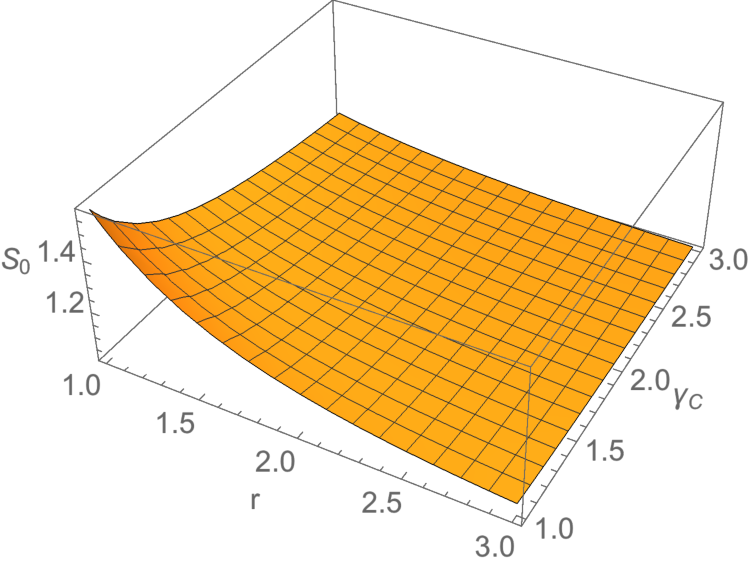
\includegraphics[width=0.4\textwidth]{qubit_ass_pricing_model}
\caption{\comment{To do}}\label{fig:qubit_ass_pricing_model}
\end{figure}

\comment{What's the difference between this and the hardware cost???}

%In the limit of fast network growth, \mbox{$\gamma_N\gg 1$}, we have,
%\begin{align}
%S \approx n\cdot L_0 \cdot \chi_\text{sc}(N_0).
%\end{align}


%%%%%%%%%

